\subsection{Wyniki dla podziału na $m$ obszarów}

Ten podrozdział opisuje wyniki podziału siatki podzielonej na $m \cdot k$ partycji na $m$ partycji, z których każda
zawiera $k$ podobszarów.
Dla tej części zakładam, że podział na $m \cdot k$ partycji jest na równe, bądź niemal równe części i podaję
wyniki tylko dla podziału na $m$ partycji po $k$ podobszarów każda.
Różnica w wywołaniu algorytmu dla tej części polega na tym, że wykonywanych jest $100$ iteracji
partycjonowania na $m \cdot k$ partycji, a dla każdego z tych podziałów wykonywane jest $100$ iteracji poszukiwania
najlepszego podzielenia tych $m \cdot k$ partycji na $m$ partycji po $k$ podobszarów każda.
Jest to możliwe, ponieważ szukanie najlepszego podziału $m \cdot k$ partycji na $m$ partycji po $k$ podobszarów
ma niski koszt obliczeniowy.
Ze wszystkich wywołań wybierany jest ten podział na $m$ partycji, który ma najkrótszą długość granic.
Długość granic pod rysunkiem podawana jest dla podziału na $m$ obszarów.

Rysunek \ref{result:m:1} pokazuje partycjonowanie dla $k$ i $m$ wynoszącego $4$.
$16$ obszarów dzielone jest na $4$ partycje po $4$ podobszary każda.
Podział na $m$ obszarów nie wykazał żadnych obszarów rozproszonych - każda partycja jest całością,
a granica między obszarami jest krótka.
Wszystkie z czterech partycji mają niemal równe rozmiary, co znaczy, że wielkości partycji dla podziału (a) są
niemal idealnie równe.
\begin{figure}[h]
\centering
\begin{subfigure}{.33\textwidth}
    \centering
    \fbox{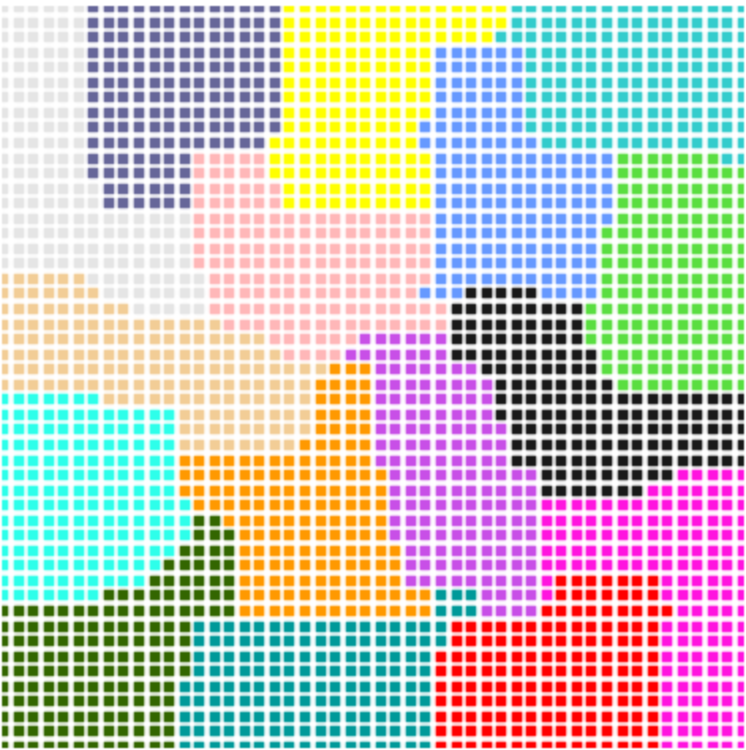
\includegraphics[width=0.7\linewidth]{images/results/m/1/mk}}
    \caption[short]{}
\end{subfigure}%
\begin{subfigure}{.33\textwidth}
    \centering
    \fbox{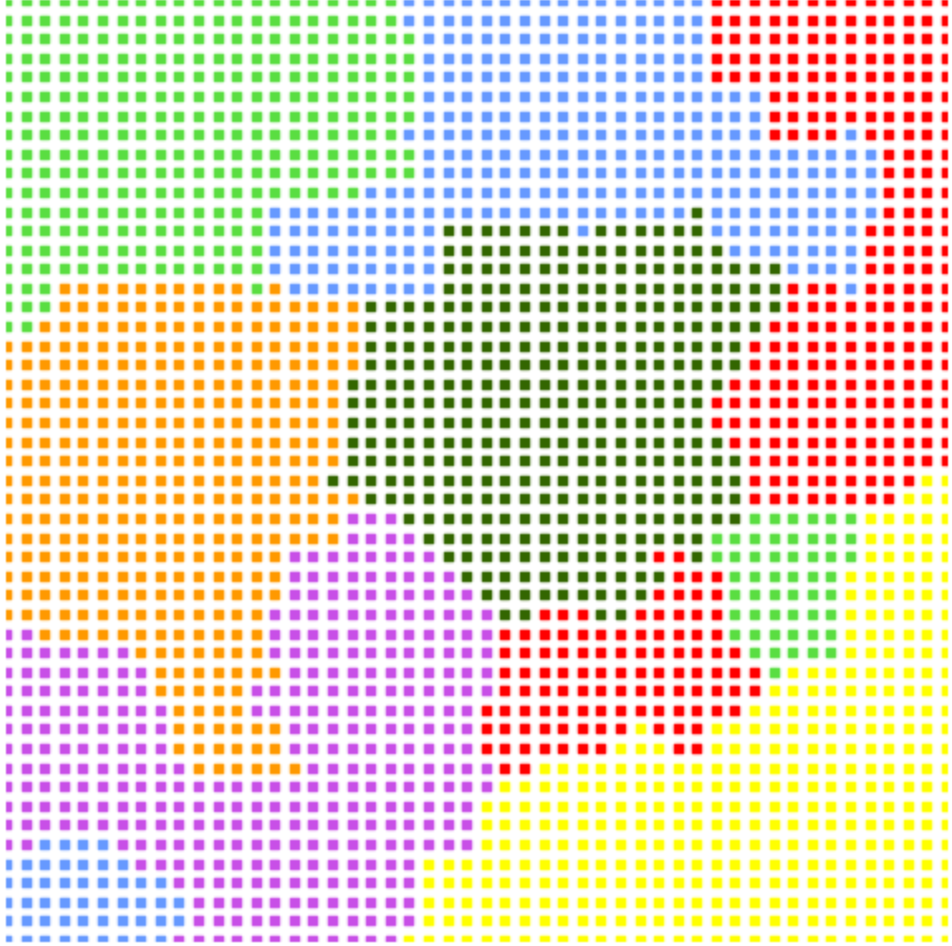
\includegraphics[width=0.7\linewidth]{images/results/m/1/m}}
    \caption[short]{}
\end{subfigure}
\begin{subfigure}{.33\textwidth}
    \centering
    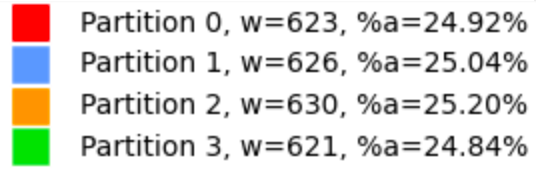
\includegraphics[width=0.9\linewidth]{images/results/m/1/results}
    \caption[short]{}
\end{subfigure}
\caption{Siatka $50$x$50$. $k$ i $m$ wynosi $4$.
Sumaryczna długość granic dla tego wyniku wynosi $146$.
Wybór najlepszego rezultatu wedle kryterium najmniejszej długości granic.
Odchylenie standardowe wielkości pól wynosi $0.1356$.}
\label{result:m:1}
\end{figure}
\begin{figure}[h]
\centering
\begin{subfigure}{.33\textwidth}
    \centering
    \fbox{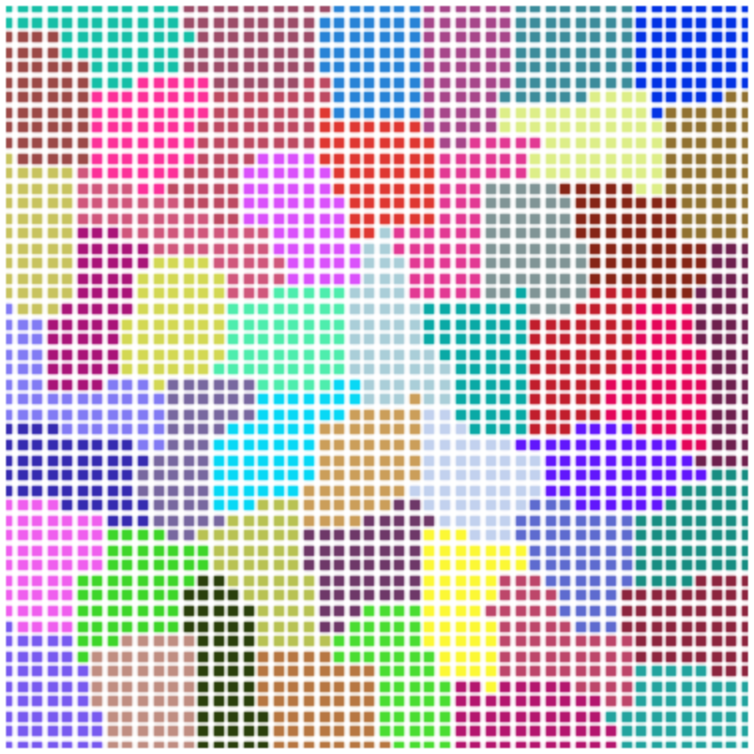
\includegraphics[width=0.7\linewidth]{images/results/m/2/mk}}
    \caption[short]{}
\end{subfigure}%
\begin{subfigure}{.33\textwidth}
    \centering
    \fbox{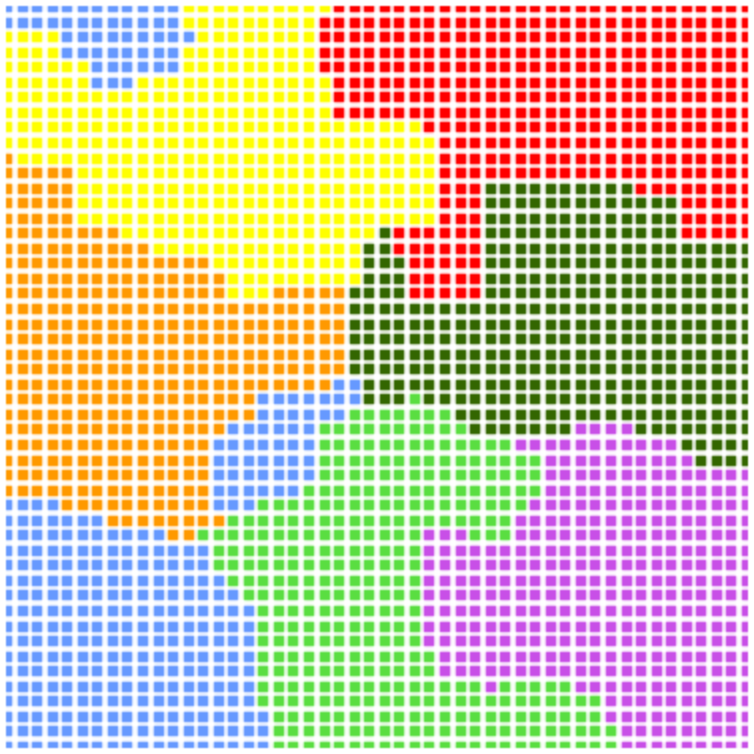
\includegraphics[width=0.7\linewidth]{images/results/m/2/m}}
    \caption[short]{}
\end{subfigure}
\begin{subfigure}{.33\textwidth}
    \centering
    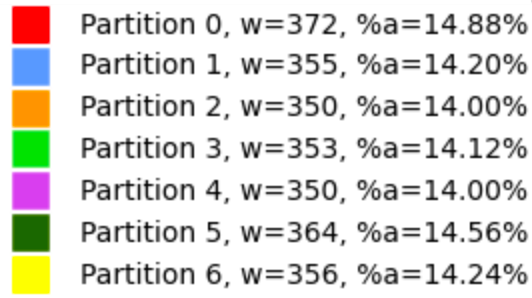
\includegraphics[width=0.9\linewidth]{images/results/m/2/results}
    \caption[short]{}
\end{subfigure}
\caption{Siatka $50$x$50$. $k$ i $m$ wynosi $7$.
Sumaryczna długość granic dla tego wyniku wynosi $365$.
Wybór najlepszego rezultatu wedle kryterium najmniejszej długości granic.
Odchylenie standardowe wielkości pól wynosi $0.2996$.}
\label{result:m:2}
\end{figure}
\begin{figure}[h]
\centering
\begin{subfigure}{.33\textwidth}
    \centering
    \fbox{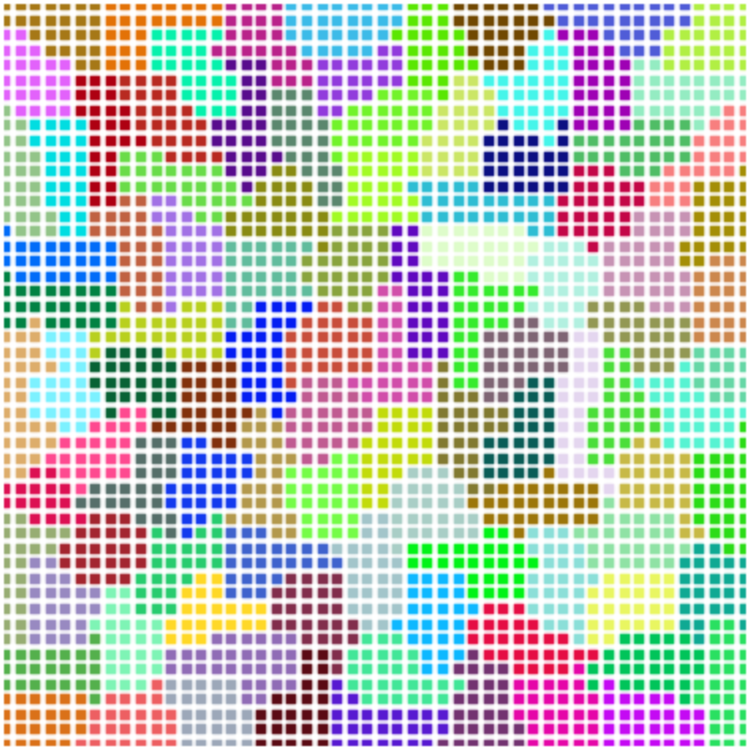
\includegraphics[width=0.7\linewidth]{images/results/m/3/mk}}
    \caption[short]{}
\end{subfigure}%
\begin{subfigure}{.33\textwidth}
    \centering
    \fbox{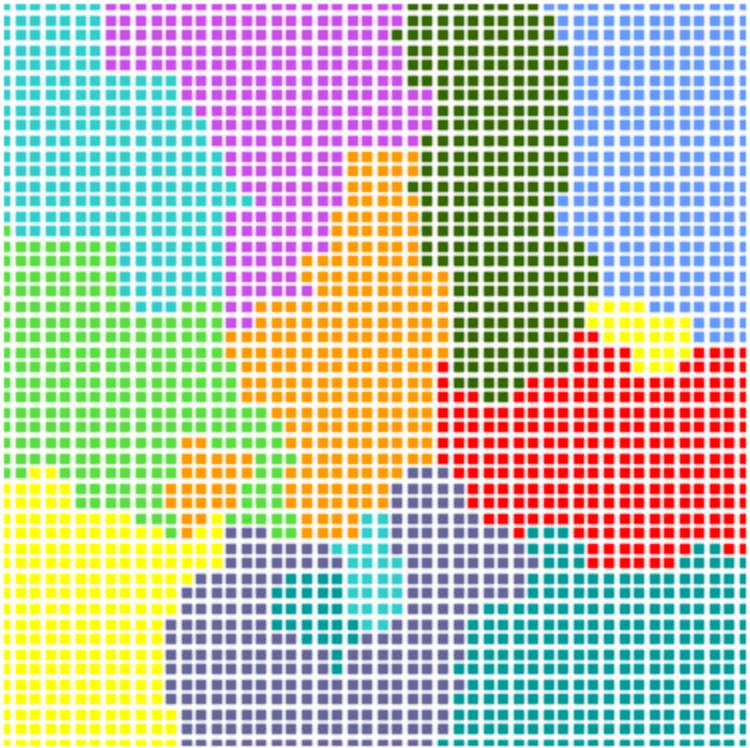
\includegraphics[width=0.7\linewidth]{images/results/m/3/m}}
    \caption[short]{}
\end{subfigure}
\begin{subfigure}{.33\textwidth}
    \centering
    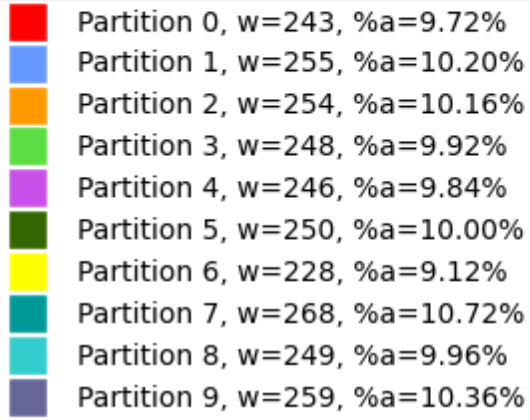
\includegraphics[width=0.9\linewidth]{images/results/m/3/results}
    \caption[short]{}
\end{subfigure}
\caption{Siatka $50$x$50$. $k$ i $m$ wynosi $10$.
Sumaryczna długość granic dla tego wyniku wynosi $509$.
Wybór najlepszego rezultatu wedle kryterium najmniejszej długości granic.
Odchylenie standardowe wielkości pól wynosi $0.4$.}
\label{result:m:3}
\end{figure}
\begin{figure}[h]
\centering
\begin{subfigure}{.33\textwidth}
    \centering
    \fbox{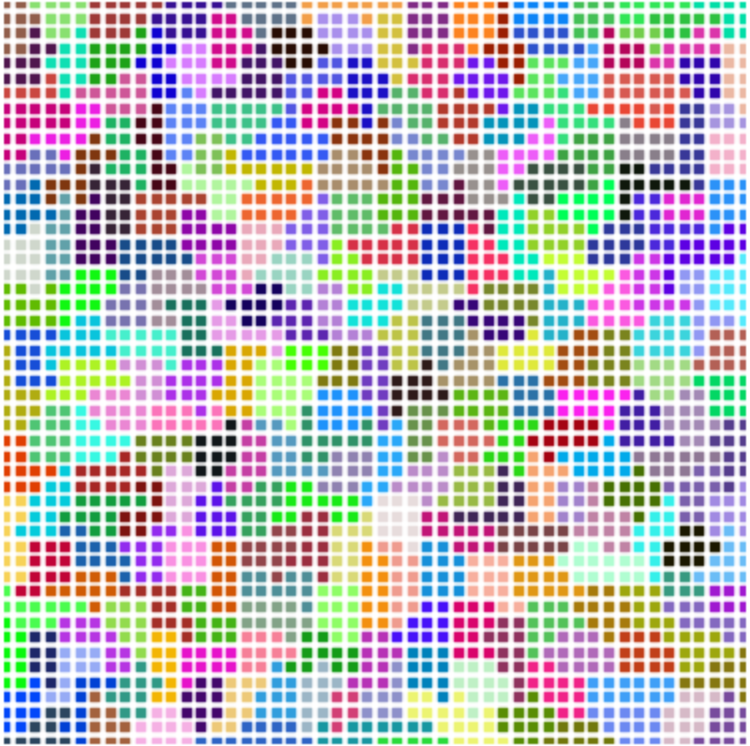
\includegraphics[width=0.7\linewidth]{images/results/m/4/mk}}
    \caption[short]{}
\end{subfigure}%
\begin{subfigure}{.33\textwidth}
    \centering
    \fbox{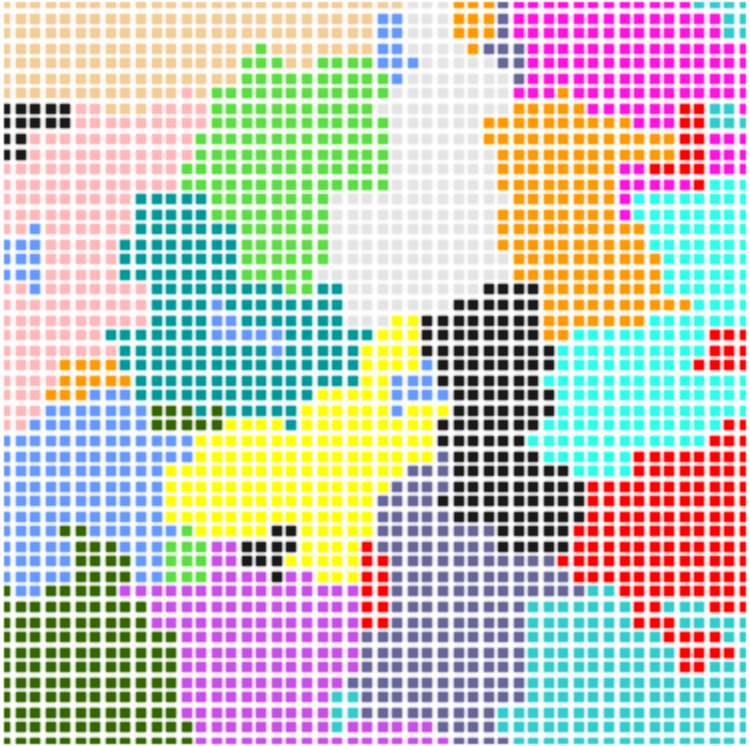
\includegraphics[width=0.7\linewidth]{images/results/m/4/m}}
    \caption[short]{}
\end{subfigure}
\begin{subfigure}{.33\textwidth}
    \centering
    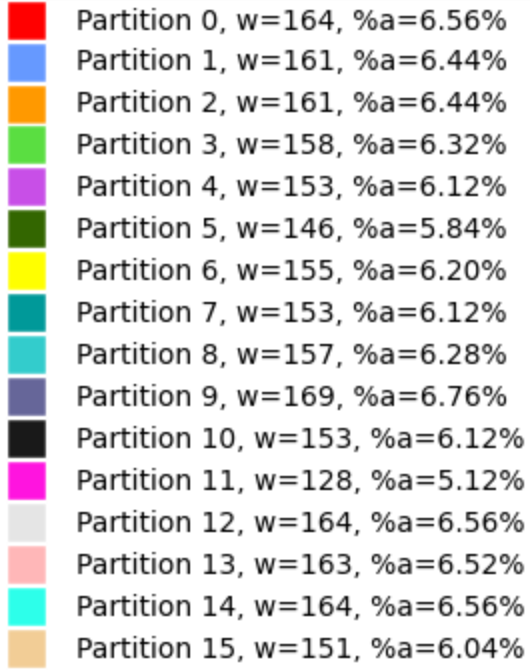
\includegraphics[width=0.9\linewidth]{images/results/m/4/results}
    \caption[short]{}
\end{subfigure}
\caption{Siatka $50$x$50$. $k$ i $m$ wynosi $16$.
Sumaryczna długość granic dla tego wyniku wynosi $793$.
Wybór najlepszego rezultatu wedle kryterium najmniejszej długości granic.
Odchylenie standardowe wielkości pól wynosi $0.3742$.}
\label{result:m:4}
\end{figure}
\Floatbarrier


Rysunek \ref{result:m:2} pokazuje partycjonowanie dla $k$ i $m$ wynoszącego $7$.
$49$ obszarów dzielone jest na $7$ partycji po $7$ podobszarów każda.
Po raz pierwszy widoczne są obszary rozproszone, są one jednak pojedyncze i tylko dla partycji $1$.
Wszystkie z siedmiu partycji mają niemal równe rozmiary, to znaczy, że wielkości partycji dla podziału (a) są
niemal idealnie równe.
Rysunek \ref{result:m:3} pokazuje partycjonowanie dla $k$ i $m$ wynoszącego $10$.
$100$ obszarów dzielone jest na $10$ partycji po $10$ podobszarów każda.
Wraz z liczbą obszarów rośnie liczba partycji rozproszonych, nie jest ona jednak duża.
Jest to tylko kilka pojedynczych obszarów.
Podział można uznać za udany.
Rysunek \ref{result:m:4} pokazuje partycjonowanie dla $k$ i $m$ wynoszącego $16$.
$256$ obszarów dzielone jest na $16$ partycji po $16$ podobszarów każda.
Widoczne jest analogiczne zachowanie jak wcześniej, rośnie liczba rozproszonych obszarów, jest ich jednak
mniej niż $10\%$.

Można zaobserwować, że wraz z liczbą partycji rośnie liczba partycji rozproszonych, nie jest to jednak bardzo intensywne
zjawisko.
Eksperymenty wykazały, że w celu znalezienia najlepszego partycjonowania lepiej wykonać więcej
podziałów na $m \cdot k$ partycji ($100$ prób), a następnie
dla każdego z nich podobną liczbę partycjowań na $m$ partycji po $k$ obszarów ($100$ prób),
niż wykonać mniej podziałów na $m \cdot k$ partycji ($1$-$10$ prób) i dla każdego
z nich znacznie więcej partycjowań na $m$ partycji po $k$ obszarów ($1000$-$3000$ prób).
Druga opcja jest możliwa, ponieważ wyliczanie partycjowań na $m$ partycji po $k$ obszarów jest bardzo mało kosztowne
obliczeniowo, ale dla tej opcji występuje znacznie więcej obszarów rozproszonych i długość granic między partycjami
jest większa.


\begin{figure}[h]
\centering
\begin{subfigure}{.33\textwidth}
    \centering
    \fbox{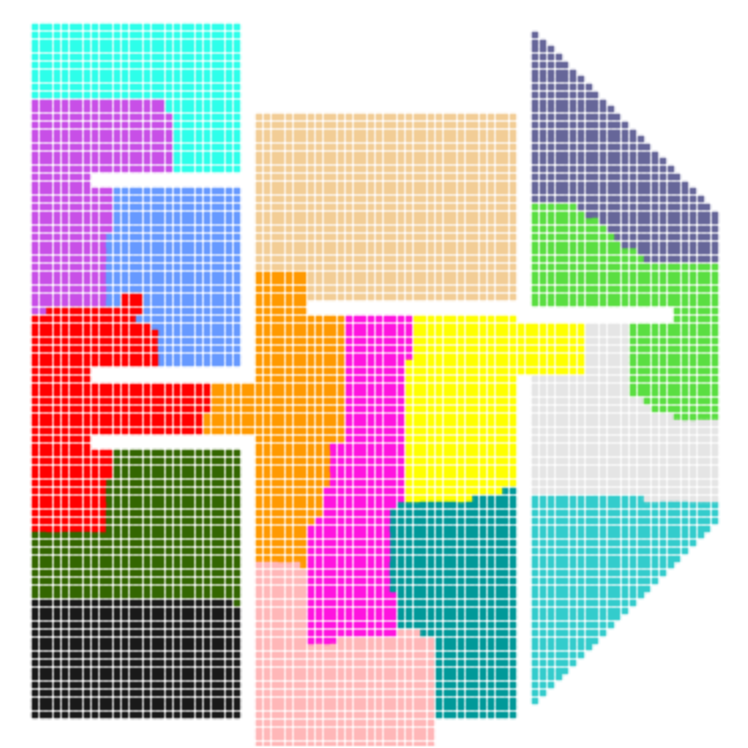
\includegraphics[width=0.9\linewidth]{images/results/m/5/mk}}
    \caption[short]{}
\end{subfigure}%
\begin{subfigure}{.33\textwidth}
    \centering
    \fbox{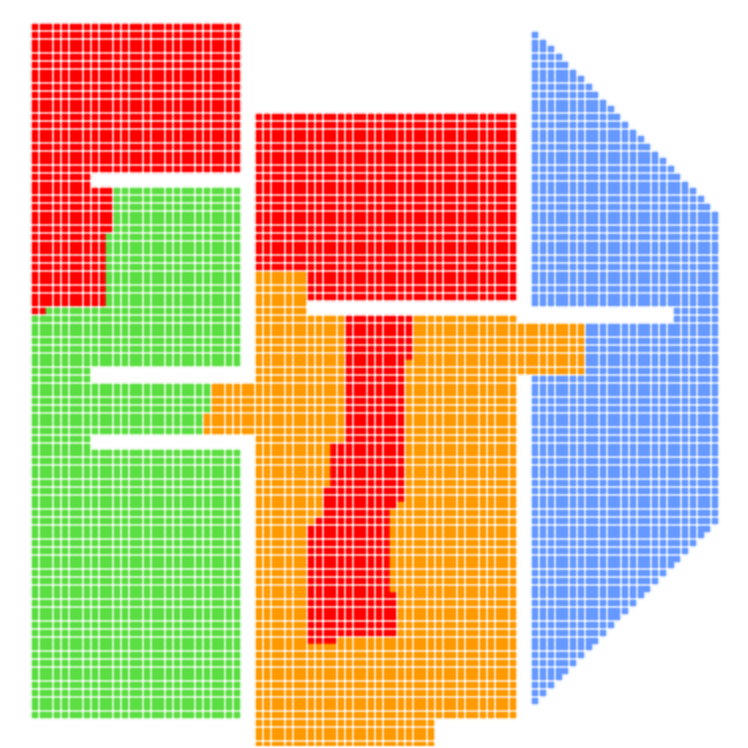
\includegraphics[width=0.9\linewidth]{images/results/m/5/m}}
    \caption[short]{}
\end{subfigure}
\begin{subfigure}{.33\textwidth}
    \centering
    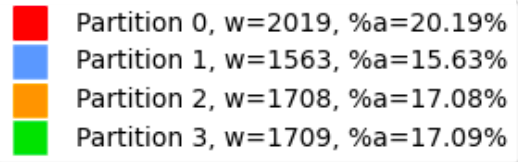
\includegraphics[width=0.9\linewidth]{images/results/m/5/results}
    \caption[short]{}
\end{subfigure}
\caption{Siatka $100$x$100$. $k$ i $m$ wynosi $16$.
Sumaryczna długość granic dla tego wyniku wynosi $200$.
Obszary wyłączone z obliczeń nie są mapowane na wierzchołki.
Wybór najlepszego rezultatu wedle kryterium najmniejszej długości granic.
Odchylenie standardowe wielkości pól wynosi $1.6641$.}
\label{result:m:5}
\end{figure}

Na rysunku \ref{result:m:5} przedstawiono partycjonowanie siatki, która wystąpiła również na rysunku \ref{result:18}.
W tym wypadku obszary nie muszą być ''zwarte'' w celu uzyskania niskiej wartości długości granic, ponieważ
ściany ograniczają wartość tego parametru.
